    % Apresentações em widescreen. Outros valores possíveis: 1610, 149, 54, 43 e 32.
% Por padrão, as apresentações são no formato 4:3 (sem o aspectratio).
\documentclass[aspectratio=169]{beamer}	 	

\renewcommand\textbullet{\ensuremath{\bullet}}

\usetheme{Pittsburgh}
\usecolortheme{default}
\usefonttheme[onlymath]{serif}			% para fontes matemáticas
% Enconte mais temas e cores em http://www.hartwork.org/beamer-theme-matrix/ 
% Veja também http://deic.uab.es/~iblanes/beamer_gallery/index.html
% Customizações de Cores: fg significa cor do texto e bg é cor do fundo
\setbeamercolor{normal text}{fg=black}
\setbeamercolor{alerted text}{fg=red}
\setbeamercolor{author}{fg=black}
\setbeamercolor{institute}{fg=black}
\setbeamercolor{date}{fg=black}
\setbeamercolor{frametitle}{fg=black}
\setbeamercolor{framesubtitle}{fg=brown}
\setbeamercolor{block title}{bg=black, fg=white}	%Cor do título
\setbeamercolor{block body}{bg=gray, fg=black}	%Cor do texto (bg= fundo; fg=texto)
\setbeamercolor{section in toc}{fg=black}
\setbeamercolor{section number projected}{bg=white,fg=black}
\setbeamercolor{titlelike}{fg=black}
% ---
% PACOTES
% ---
\usepackage[alf]{abntex2cite}	% Citações padrão ABNT
\usepackage[brazil]{babel}		% Idioma do documento
\usepackage{color}				% Controle das cores
\usepackage[T1]{fontenc}		% Selecao de codigos de fonte.
\usepackage{graphicx}			% Inclusão de gráficos
\usepackage[utf8]{inputenc}		% Codificacao do documento (conversão automática dos acentos)
\usepackage{txfonts}			% Fontes virtuais
\usepackage{bmpsize}
\usepackage[absolute,overlay]{textpos}
% ---

% --- Informações do documento ---
\title{Avaliando Sistemas de Detecção de Intrusão em uma Rede Acadêmica}
\author{Glenon Mateus Barbosa Araújo}
\institute{Trabalho de Conclusão de Curso}
\date{\today}
% ---

% ----------------- INÍCIO DO DOCUMENTO --------------------------------------
\begin{document}
%\usebackgroundtemplate{
\includegraphics[width=1.5cm,height=\paperheight]{imagens/imagem.png}}
% ----------------- NOVO SLIDE --------------------------------
\begin{frame}
\begin{minipage}{\linewidth}
  \centering
  \begin{tabular}{cc}
    \begin{tabular}{c}
      \textbf{Universidade Federal do Pará} \\ 
      \textbf{Faculdade de Computação} \\
      \textbf{Bacharelado em Ciência da Computação}
    \end{tabular}
    &
    \begin{tabular}{c}
     
\includegraphics[width=2.2cm]{imagens/ufpa-logo.jpeg}
    \end{tabular}
  \end{tabular}
\end{minipage}
\titlepage
\end{frame}
% ----------------- NOVO SLIDE --------------------------------
\begin{frame}{Agenda}
  \tableofcontents
\end{frame}
% ----------------- NOVO SLIDE --------------------------------
\section{Introdução}
\begin{frame}{Introdução}
    \begin{itemize}
        \item Internet = conjuntos de redes heterogênea;
        \item maior a complexidade, maior numero de vulnerabilidades;
        \item CERT.br - 722205 incidentes reportados (Scan, Fraude, DoS, Worm);
        \item \textit{Firewall} não é uma solução definitiva; 
        \item Necessidade de outras ferramentas (flexibilidade, eficiência, desempenho, administração simplificada);
    \end{itemize}
\end{frame}
% ----------------- NOVO SLIDE --------------------------------
\subsection{Motivação}
\begin{frame}{Introdução}
    \framesubtitle{Motivação}
    \begin{itemize}
        \item Necessidade de implantação de um IDS;
        \item Uso gratuito;
        \item Ferramentas Snort e Suricata;
    \end{itemize}
\end{frame}
% ----------------- NOVO SLIDE --------------------------------
\subsection{Objetivos}
\begin{frame}{Introdução}
    \framesubtitle{Objetivos}
    \begin{itemize}
        \item \textbf{Geral:} 
            \begin{itemize}
                \item Avaliar e fazer um comparativo;
            \end{itemize}
        \item \textbf{Secundário:} 
            \begin{itemize}
                \item Apresentar conceitos sobre segurança da informação; 
                \item Descrever problemas relacionados a ataques envolvendo redes de computadores;
                \item Descrever as ferramentas, compreendendo requisitos, características, modos de atuação e funcionalidades;
                \item Descrever o ambiente experimental;
                \item Realizar experimentos e coltar dados.
            \end{itemize}
    \end{itemize}
\end{frame}
% ----------------- NOVO SLIDE --------------------------------
\section{Segurança}
\begin{frame}{Segurança}
    \framesubtitle{Definições}
    \begin{itemize}
        \item \textbf{Incidente de Segurança:} Qualquer evento oposto a segurança;
        \item \textbf{Ativo:} Qualquer coisa que tenha valor para a organização e para seus negócios;
        \item \textbf{Ameaça:} Qualquer evento que explore vulnerabilidades;
        \item \textbf{Vulnerabilidade:} Qualquer fraqueza que possa ser explorada;
        \item \textbf{Risco:} Probabilidade de uma ameaça se concretizar;
        \item \textbf{Ataque:} Qualquer ação que comprometa a segurança;
        \item \textbf{Impacto:} Consequências de um evento;
    \end{itemize}
\end{frame}
% ----------------- NOVO SLIDE --------------------------------
\begin{frame}{Segurança}
    \framesubtitle{Pilares da Segurança}
    \begin{itemize}
        \item \textbf{Confidencialidade:} ligado à privacidade, acesso somente por pessoas ou grupos autorizados;
        \item \textbf{Integridade:} Informação ter valor correto, inviolabilidade da informação;
        \item \textbf{Disponibilidade:} relacionada ao acesso à informação; 
        \item \textbf{Autenticidade:} garantia de que a informação foi elaborado ou distribuído pelo autor;
        \item \textbf{Legalidade:} garantia de que ações sejam realizadas em conformidade com os preceitos legais;
        \item \textbf{Não Repúdio:} emissor de uma mensagem não pode negar que a enviou;
        \item \textbf{Privacidade:} habilidade de uma pessoa controlar a exposição e a disponibilidade de informações acerca de si;
    \end{itemize}
\end{frame}
% ----------------- NOVO SLIDE --------------------------------
\begin{frame}{Segurança}
    \framesubtitle{Ataques Comuns}
    \begin{itemize}
        \item \textbf{\textit{Scanner:}} varrer a rede a procura de um alvo em potencial; 
            \begin{itemize}
                \item \textbf{\textit{Portscanner}:} verifica quais portas estão abertas no alvo;
                \item \textbf{Vulnerabilidade:} verifica se o serviço está executando uma versão com alguma vulnerabilidades;
            \end{itemize}
        \item \textbf{Negação de Serviço:} deixar um serviço ou recurso indisponível;
    \end{itemize}
\end{frame}
% ----------------- NOVO SLIDE --------------------------------
\section{Sistemas de Detecção de Intrusão}
\begin{frame}{Sistema de Detecção de Intrusão}
    \framesubtitle{Definição}
    \begin{itemize}
        \item \textbf{IDS:} Monitoramento de eventos que ocorrem em redes e sistemas computacionais, analisando sinais de possíveis ataques, alertando os administradores;
        \item \textbf{IPS:} todas as funcionalidades do IDS, porém é capaz de deter os incidentes;
    \end{itemize}
\end{frame}
% ----------------- NOVO SLIDE --------------------------------
\subsection{Tipos}
\begin{frame}{Sistemas de Detecção de Intrusão}
    \framesubtitle{Tipos}
    \begin{itemize}
        \item \textbf{HIDS:} sensor é instalado no \textit{host}; verificação de informações relativas aos eventos e registros de \textit{logs} e sistemas de arquivos;
        \item \textbf{NIDS:} sensor é instalado na rede; monitora e analisa o trafego do segmento de rede;
            \begin{itemize}
                \item \textbf{Passivo:} monitora copias dos pacotes da rede (espelhamento)
                \item \textbf{Ativo:} trafego passa através do sensor (atuação similar a de um \textit{firewall})
            \end{itemize}
        \item \textbf{SDID:} envio de alertas para um servidor central (gerencia)
        \item \textbf{Forma de Detecção:}
            \begin{itemize}
                \item \textbf{Assinaturas:} compara com uma base de assinaturas de ataques conhecidos;
                \item \textbf{Anomalias:} determina um comportamento normal da rede, qualquer desvio desse comportamento gera alertas;
            \end{itemize}
    \end{itemize}
\end{frame}
% ----------------- NOVO SLIDE --------------------------------
\subsection{Ferramentas}
\begin{frame}{Sistemas de Detecção de Intrusão}
    \framesubtitle{Ferramentas}
    \begin{minipage}{\linewidth}
        \centering
        \begin{tabular}{cc}
            \begin{tabular}{l}
                \textbf{Snort} \\
                \\
                \hline
                \\
                Linguaguem C; \\
                Lançamento em 1998; \\
                Baseado em assinaturas e anomalias; \\
                \textit{Sniffer}; \textit{Packet Logger}; NIDS; \\
            \end{tabular}
            &
            \begin{tabular}{c}
                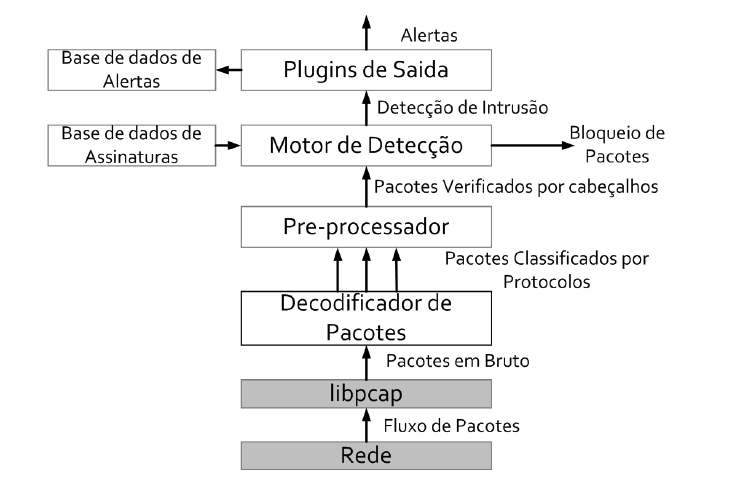
\includegraphics[width=8cm]{imagens/arquitetura-snort.png}
            \end{tabular}
        \end{tabular}
    \end{minipage}
\end{frame}
% ----------------- NOVO SLIDE --------------------------------
\begin{frame}{Sistemas de Detecção de Intrusão}
    \framesubtitle{Ferramentas}
    \begin{minipage}{\linewidth}
        \centering
        \begin{tabular}{cc}
            \begin{tabular}{l}
                \textbf{Suricata} \\
                \\
                \hline
                \\
                Lançamento em 2010; \\
                Baseado em assinaturas e anomalias; \\
                Arquitetura inspirada no Snort; \\
                \textit{Multithread}; \\
                \textit{Sniffer}; \textit{Packet Logger}; NIDS; NSM; \\
            \end{tabular}
            &
            \begin{tabular}{c}
                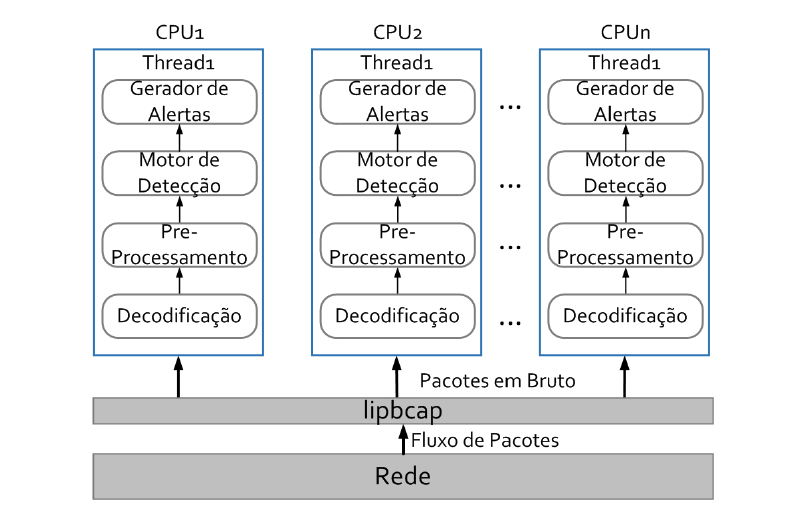
\includegraphics[width=8cm]{imagens/arquitetura-suricata.png}
            \end{tabular}
        \end{tabular}
    \end{minipage}
\end{frame}
% ----------------- NOVO SLIDE --------------------------------
\section{IDS em um Cenário Real}
\begin{frame}{IDS em um Cenário Real}
    \framesubtitle{Cenário de Testes}
    \begin{minipage}{\linewidth}
        \begin{tabular}{cc}
            \begin{tabular}{l}
                Taxa de Transferência = 800 Mbps; \\
                Quantidade de usuário indeterminado;
            \end{tabular}
            &
            \begin{tabular}{l}
                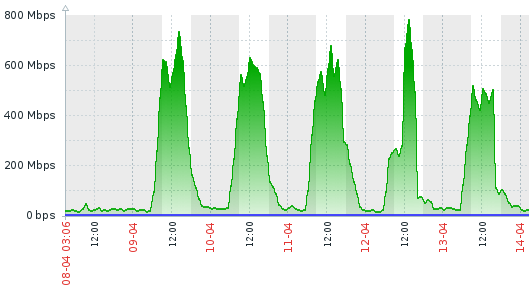
\includegraphics[width=7cm]{imagens/trafego-rede.png}
            \end{tabular}
        \end{tabular}
    \end{minipage}
\end{frame}
% ----------------- NOVO SLIDE --------------------------------
\subsection{Testes Realizados}
\begin{frame}{IDS em um Cenário Real}
    \framesubtitle{Infraestrutura}
    \begin{minipage}{\linewidth}
        \begin{tabular}{c}
            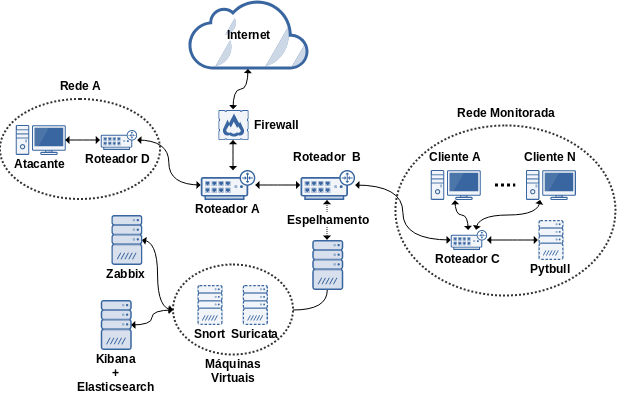
\includegraphics[width=11cm]{imagens/infra.png}
        \end{tabular}
    \end{minipage}
\end{frame}
% ----------------- NOVO SLIDE --------------------------------
\subsection{Resultados}
\begin{frame}{IDS em um Cenário Real}
    \framesubtitle{Teste Realizados}
    \begin{itemize}
        \item \textbf{\textit{Portscanner}}
        \begin{itemize}
            \item nmap -F 200.239.72.19
            \item nmap -A 200.239.72.19
            \item execução dos comandos via \textit{script}
        \end{itemize}
        \item \textbf{\textit{Scan} de Vulnerabilidade} (OpenVAS)
        \item \textbf{DoS} (Metasploit Framework)
            \begin{itemize}
                \item use auxiliary/dos/tcp/synflood
            \end{itemize}        
        \item \textbf{Pytbull}
    \end{itemize}
\end{frame}
% ----------------- NOVO SLIDE --------------------------------
\begin{frame}{IDS em um Cenário Real}
    \framesubtitle{Resultados}
    \begin{minipage}{\linewidth}
        \begin{tabular}{cc}
            \begin{tabular}{l}
                \textbf{nmap -F} \\ 
                \\
                \hline
                \\
                Total = 62 alertas; \\
                100\% do Snort;
            \end{tabular}
            &
            \begin{tabular}{c}
                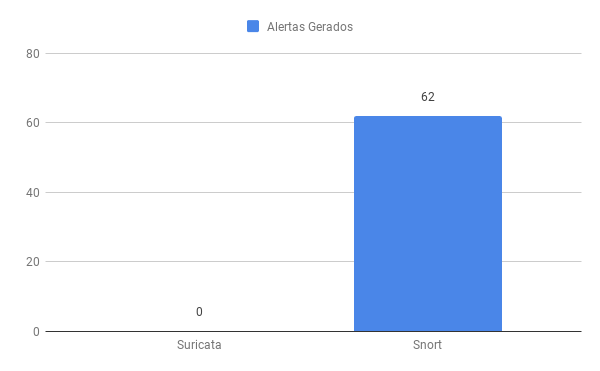
\includegraphics[width=9cm]{imagens/teste-nmap-fast.png}
            \end{tabular}
        \end{tabular}
    \end{minipage}
\end{frame}
% ----------------- NOVO SLIDE --------------------------------
\begin{frame}{IDS em um Cenário Real}
    \framesubtitle{Resultados}
    \begin{minipage}{\linewidth}
        \begin{tabular}{cc}
            \begin{tabular}{l}
                \textbf{nmap -A} \\ 
                \\
                \hline
                \\
                Total = 210 alertas; \\
                50.5\% Suricata; \\
                49.5\% Snort;
            \end{tabular}
            &
            \begin{tabular}{c}
                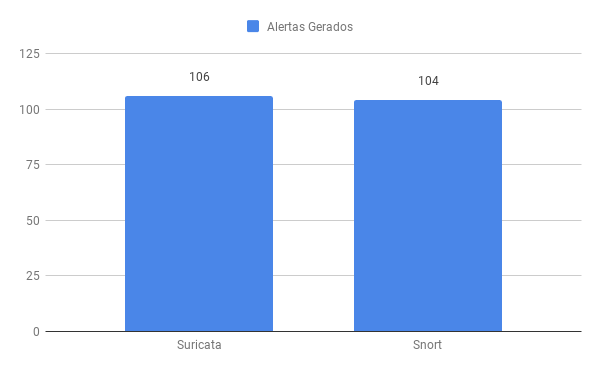
\includegraphics[width=9cm]{imagens/teste-nmap-all.png}
            \end{tabular}
        \end{tabular}
    \end{minipage}
\end{frame}
% ----------------- NOVO SLIDE --------------------------------
\begin{frame}{IDS em um Cenário Real}
    \framesubtitle{Resultados}
    \begin{minipage}{\linewidth}
        \begin{tabular}{cc}
            \begin{tabular}{l}
                \textbf{OpenVAS} \\ 
                \\
                \hline
                \\
                Total = 3071 alertas; \\
                69.74\% Suricata; \\
                30.26\% Snort;
            \end{tabular}
            &
            \begin{tabular}{c}
                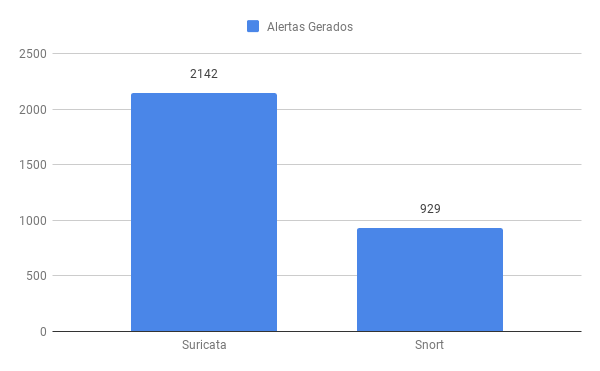
\includegraphics[width=9cm]{imagens/teste-openvas.png}
            \end{tabular}
        \end{tabular}
    \end{minipage}
\end{frame}
% ----------------- NOVO SLIDE --------------------------------
\begin{frame}{IDS em um Cenário Real}
    \framesubtitle{Resultados}
    \begin{minipage}{\linewidth}
        \begin{tabular}{cc}
            \begin{tabular}{l}
                \textbf{Taxa de detecção} \\ 
                \\
                \hline
                \\
                Total = 47778 alertas; \\
                62.99\% Suricata; \\
                37.01\% Snort;
            \end{tabular}
            &
            \begin{tabular}{c}
                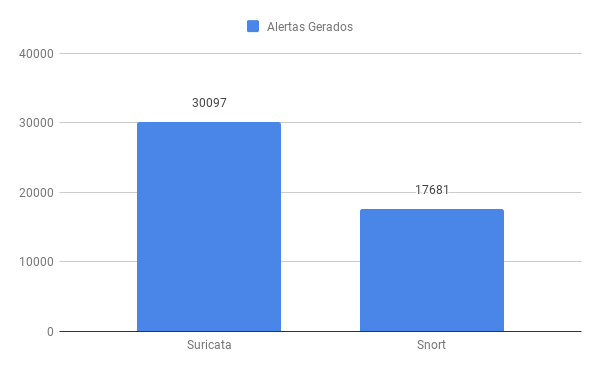
\includegraphics[width=9cm]{imagens/teste-taxa-de-deteccao.png}
            \end{tabular}
        \end{tabular}
    \end{minipage}
\end{frame}
% ----------------- NOVO SLIDE --------------------------------
\begin{frame}{IDS em um Cenário Real}
    \framesubtitle{Resultados}
    \begin{minipage}{\linewidth}
        \begin{tabular}{cc}
            \begin{tabular}{c}
                \textbf{Suricata} \\
                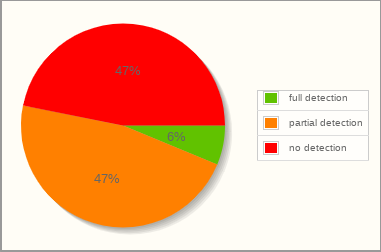
\includegraphics[width=6cm]{imagens/suricata-pytbull-report.png}
            \end{tabular}
            &
            \begin{tabular}{c}
                \textbf{Snort} \\
                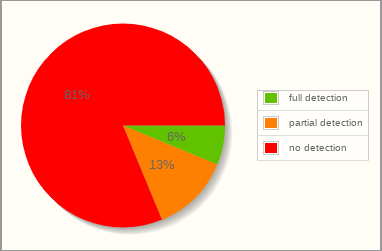
\includegraphics[width=6cm]{imagens/snort-pytbull-report.png}
            \end{tabular}
        \end{tabular}
    \end{minipage}
\end{frame}
% ----------------- NOVO SLIDE --------------------------------
\begin{frame}{IDS em um Cenário Real}
    \framesubtitle{Resultados}
    \begin{minipage}{\linewidth}
        \begin{tabular}{c}
            \begin{tabular}{c}
                \textbf{Suricata} \\
                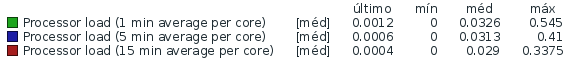
\includegraphics[width=12cm]{imagens/suricata-cpu-load.png} \\
                
\includegraphics[width=10cm]{imagens/suricata-memory-usage.png} \\
                \\
                \hline
                \\
                \textbf{Snort} \\
                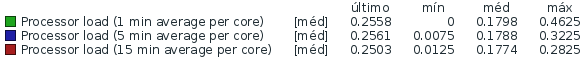
\includegraphics[width=12cm]{imagens/snort-cpu-load.png} \\
                
\includegraphics[width=10cm]{imagens/snort-memory-usage.png} \\
            \end{tabular}
        \end{tabular}
    \end{minipage}
\end{frame}
% ----------------- NOVO SLIDE --------------------------------
\section{Considerações Finais}
\begin{frame}{Considerações Finais}
    \begin{itemize}
        \item Documentação do Suricata;
        \item Implantação da infraestrutura de teste;
        \item Suricata teve um melhor desempenho porém não recomendado;
        \item Analisar as ferramentas tendo como foco a precisão (falsos positivos e falsos negativos);
    \end{itemize}
\end{frame}
\end{document}
